\documentclass[11pt]{article}

% ACL 2023 format requirements  
\usepackage[final]{acl}   % Use [final] for camera-ready

% ----- Standard ACL template packages -----
\usepackage{times}
\usepackage{latexsym}
\usepackage[T1]{fontenc}
\usepackage[utf8]{inputenc}
\usepackage{microtype}
\usepackage{inconsolata}
\usepackage{graphicx}
\usepackage{amsmath}
\usepackage{amssymb}
\usepackage{booktabs}   % for \toprule, \midrule, \bottomrule
\usepackage{tabularx}   % for X column
\usepackage{array}      % for >{\raggedright\arraybackslash} in X
\usepackage{multirow}   % for \multirow command
% Preamble (once):
\usepackage{enumitem}
\usepackage{subcaption}

% Make X-columns vertically centered (instead of top-aligned p{})
\renewcommand\tabularxcolumn[1]{m{#1}}

% Optional: tell LaTeX where figures may live. Put your image in figs/
\graphicspath{{figs/}}

\title{On Multi-Task Cross-Domain Pre-training for Graph Neural Networks}

\author{
  Alon Bebchuk (ID: 314023516), 
  Ben Cohen (ID: 323855288), 
  and Tim Kushmaro (ID: 212052708) \\
}

\begin{document}
\maketitle

% -------------------------
% Abstract (max 150 words)
% -------------------------
\begin{abstract}\normalfont\normalsize
While GNN pre-training approaches suggest potential for cross-domain performance improvements, practitioners report inconsistent results. We challenge this through systematic evaluation of 96 controlled experiments across 6 domains and 8 pre-training schemes. Our analysis reveals a fundamental asymmetry: \textbf{computational efficiency gains vary by domain-scheme combinations}, while \textbf{performance improvements are selective}, requiring precise matching. We identify and illustrate four predictable failure patterns with concrete examples and establish evidence-based deployment protocols. This framework transforms GNN pre-training from trial-and-error into systematic optimization through detailed efficiency and performance analysis.
\end{abstract}

\textbf{Keywords:} graph neural networks, pre-training, transfer learning, multi-task learning, computational efficiency, systematic evaluation, domain adaptation, failure analysis

\textbf{Code and Data:} Full implementations, models, and reproducible experiments available at \\\url{https://github.com/alonbebchuk/GNN-Pretraining.git}

\section{Introduction}
Graph Neural Networks (GNNs) are widely used for learning representations from relational data across diverse domains including molecules, proteins, citation networks, and knowledge graphs \citep{zhou2020graph}.
Unlike computer vision and NLP, where systematic pre-training is foundational \citep{he2016deep,devlin2019bert}, GNNs are still commonly trained from scratch per task and domain.
Prior GNN pre-training work typically focuses on either a single pretext task or a single domain \citep{hu2019strategies}, leaving the core research question unanswered: \textbf{How does multi-task cross-domain training transfer to different domains and tasks?}

We address this through a comprehensive empirical evaluation of multi-task, cross-domain GNN pre-training across 96 controlled experiments compared against from-scratch training baselines. Our systematic approach reveals fundamental asymmetries in transfer effectiveness and establishes evidence-based guidelines for practitioners.

\paragraph{Why this matters.}
GNN pre-training demonstrates computational and performance potential that can be systematically unlocked through principled optimization.
First, \textbf{computational efficiency gains} vary significantly by domain-scheme combinations, with clear efficiency clustering and domain-specific optimization patterns.
Second, \textbf{selective performance improvements} require precise domain-scheme matching, with notable gains achieved through systematic combinations.
\paragraph{Key Contributions.}
We establish: (1) \textbf{Systematic Evaluation Framework} - 96 controlled experiments revealing efficiency and performance patterns, (2) \textbf{Parameter-Performance Disconnect} - fundamental gap between parameter reduction and actual speedups, (3) \textbf{Evidence-Based Guidelines} - empirical matrices for reliable domain-scheme selection, and (4) \textbf{Failure Mode Taxonomy} - predictable patterns enabling systematic avoidance strategies.

\section{Related Work}

\paragraph{Graph pre-training approaches.} Recent comprehensive surveys \citep{xie2022self,liu2022graph} categorize self-supervised graph learning approaches including information-theoretic methods \citep{velickovic2019dgi,sun2020infograph}, generative masking \citep{hu2019strategies}, contrastive approaches \citep{you2020graphcl,hou2022graphmae}, and large-scale frameworks \citep{qiu2020gcc,liu2022graphmvp}. However, these typically evaluate single methods on specific domains without systematic multi-task or cross-domain analysis.

\paragraph{Multi-task learning in graphs.} While multi-task learning \citep{caruana1997multitask} and transfer learning \citep{pan2010survey} benefit computer vision and NLP, their application to graph pre-training remains understudied. Prior work identifies gradient interference issues and proposes solutions like PCGrad \citep{yu2020pcgrad}, but lacks comprehensive evaluation of multi-task graph pre-training effectiveness across domains.

\paragraph{Our contributions.} We provide the first systematic evaluation of multi-task graph pre-training across domains, revealing efficiency-performance asymmetries and establishing evidence-based deployment protocols with failure mode analysis.


\section{Methodology}

We evaluate 96 controlled experiments across molecular (MUTAG, PROTEINS, NCI1, ENZYMES) and citation (Cora, CiteSeer) datasets \citep{tudataset,sen2008collective} (see Appendix A.5 for data processing details). Task types: Graph Classification (GC), Node Classification (NC), Link Prediction (LP). Transfer strategies: Linear Probing (LIN, frozen backbone) vs Full Fine-tuning (FT, all parameters). 3 seeds for statistical reliability (see Appendix A.6 for evaluation protocol).

\paragraph{Experimental design.} Architecture: domain-adaptive encoders, 5-layer GIN backbone \citep{xu2019how}, task-specific heads (see Appendix A.1 for architecture specifications). Six pre-training objectives: node masking \citep{hou2022graphmae}, link prediction \citep{liben2007link}, contrastive learning \citep{you2020graphcl}, graph properties \citep{newman2003structure}, domain adversarial training \citep{ganin2016dann} (see Appendix B for technical details). Multi-task optimization uses PCGrad \citep{yu2020pcgrad} (see Appendix A.3).

\paragraph{Pre-training schemes.} We evaluate 8 schemes with varying task complexity: \textbf{b1} (no pre-training baseline), \textbf{b2} (node masking only), \textbf{b3} (node contrastive only), \textbf{b4} (5-task: node masking, link prediction, node contrastive, graph contrastive, graph properties), \textbf{s1} (2-task: node masking, link prediction), \textbf{s2} (2-task: node contrastive, graph contrastive), \textbf{s3} (4-task: node masking, link prediction, node contrastive, graph contrastive), \textbf{s4} (5-task: s3 + graph properties), \textbf{s5} (6-task: s4 + domain adversarial). All schemes train on 4 molecular datasets except b4 (ENZYMES only). We test 8 schemes × 6 datasets × 2 transfer strategies (linear probing \citep{chen2020simple} vs full fine-tuning) = 96 pre-training experiments, compared against from-scratch baseline controls, yielding 324 total runs across 3 statistical seeds. All experiments use identical architectures and hyperparameters for fair comparison (see Appendix A.2 and C for hyperparameter details). All models are implemented using PyTorch \citep{paszke2019pytorch} and PyTorch Geometric \citep{fey2019fast}.


\paragraph{Research Questions and Contributions.} 
We address four fundamental questions:
\textbf{RQ1}: Do efficiency gains generalize universally? \textit{Answer: No - efficiency patterns are domain-scheme specific, with best overall speedups reaching 1.70x (Cora\_LP+b3) and varied time-convergence trade-offs.}
\textbf{RQ2}: When do performance gains occur? \textit{Answer: Only with precise domain-scheme matching (26.2\% success rate).}
\textbf{RQ3}: How should practitioners balance efficiency vs performance? \textit{Answer: Consult domain-scheme efficiency matrices; efficiency and performance gains exist but require careful selection.}
\textbf{RQ4}: Can failures be predicted? \textit{Answer: Yes - we identify four systematic failure patterns with predictable characteristics.}

\section{Results}

Our 96-experiment evaluation reveals fundamental asymmetries in GNN pre-training effectiveness across domains and tasks compared to from-scratch baselines.

\paragraph{RQ1 - Efficiency Gains Across Domains and Schemes.} Pre-training demonstrates varied computational advantages across different domain-scheme combinations for both transfer strategies (Tables~\ref{tab:full-finetuning} and~\ref{tab:linear-probing}). \textbf{Full fine-tuning strategy} shows notable overall speedups with CiteSeer\_NC multi-task schemes (s4: 1.54x, s5: 1.51x, s2: 1.45x, s1: 1.43x), combining both time and convergence benefits. \textbf{Linear probing strategy} shows superior overall speedups with Cora\_LP combinations (b3: 1.70x, b2: 1.68x, s2/s4: 1.67x) and CiteSeer\_NC multi-task schemes (s3: 1.61x, s2/s4: 1.57x), while providing substantial parameter reduction (2.2x-40.3x) by freezing GNN backbones.

\begin{table}[t]
\centering
\footnotesize
\setlength{\tabcolsep}{2.8pt}
\renewcommand{\arraystretch}{1.05}
\begin{tabular}{l c c c c c c c}
\toprule
\textbf{Domain} & \textbf{b2} & \textbf{b3} & \textbf{s1} & \textbf{s2} & \textbf{s3} & \textbf{s4} & \textbf{s5} \\
\midrule
\multicolumn{8}{c}{\textit{Time Per Epoch Speedup}} \\
CiteSeer\_LP & \textbf{2.18} & \textbf{1.35} & \textbf{1.92} & \textbf{2.68} & \textbf{2.27} & \textbf{1.67} & 0.85 \\
CiteSeer\_NC & \textbf{1.27} & \textbf{1.19} & \textbf{1.49} & \textbf{1.54} & \textbf{1.58} & \textbf{1.47} & \textbf{1.38} \\
Cora\_LP & 0.01 & 0.25 & 0.07 & 0.01 & 0.03 & 0.56 & 0.23 \\
Cora\_NC & \textbf{1.13} & \textbf{1.16} & \textbf{1.12} & \textbf{1.13} & 0.92 & \textbf{1.22} & 0.96 \\
ENZYMES & \textbf{1.66} & \textbf{1.43} & \textbf{1.57} & \textbf{1.92} & \textbf{1.70} & \textbf{1.63} & \textbf{1.62} \\
PTC\_MR & 0.45 & 0.89 & 0.88 & 0.42 & 0.60 & \textbf{1.19} & \textbf{1.35} \\
\midrule
\multicolumn{8}{c}{\textit{Convergence Speedup}} \\
CiteSeer\_LP & 0.43 & 0.66 & 0.42 & 0.32 & 0.34 & 0.57 & \textbf{1.26} \\
CiteSeer\_NC & 0.97 & \textbf{1.04} & 0.96 & 0.94 & 0.89 & \textbf{1.05} & \textbf{1.10} \\
Cora\_LP & \textbf{104.3} & \textbf{5.31} & \textbf{19.6} & \textbf{104.3} & \textbf{44.7} & \textbf{1.96} & \textbf{5.91} \\
Cora\_NC & 0.92 & 0.90 & 0.97 & \textbf{1.05} & \textbf{1.19} & 0.97 & \textbf{1.10} \\
ENZYMES & 0.52 & 0.64 & 0.60 & 0.46 & 0.54 & 0.54 & 0.55 \\
PTC\_MR & \textbf{2.52} & \textbf{1.12} & \textbf{1.05} & \textbf{2.70} & \textbf{1.68} & 0.72 & 0.60 \\
\midrule
\multicolumn{8}{c}{\textit{Overall Speedup (Time × Convergence)}} \\
CiteSeer\_LP & 0.93 & 0.89 & 0.80 & 0.85 & 0.77 & 0.96 & \textbf{1.07} \\
CiteSeer\_NC & \textbf{1.23} & \textbf{1.23} & \textbf{1.43} & \textbf{1.45} & \textbf{1.41} & \textbf{1.54} & \textbf{1.51} \\
Cora\_LP & \textbf{1.48} & \textbf{1.34} & \textbf{1.44} & \textbf{1.48} & \textbf{1.46} & \textbf{1.10} & \textbf{1.34} \\
Cora\_NC & \textbf{1.04} & \textbf{1.05} & \textbf{1.09} & \textbf{1.18} & \textbf{1.09} & \textbf{1.18} & \textbf{1.06} \\
ENZYMES & 0.87 & 0.91 & 0.94 & 0.88 & 0.92 & 0.87 & 0.89 \\
PTC\_MR & \textbf{1.13} & 0.99 & 0.93 & \textbf{1.13} & \textbf{1.02} & 0.85 & 0.81 \\
\bottomrule
\end{tabular}
\caption{\textbf{Full Fine-tuning Strategy} - Complete efficiency comparison vs. from-scratch full fine-tuning baseline (b1). Shows time per epoch speedup, convergence speedup, and overall speedup across domain-scheme combinations. Values >1 indicate speedup, <1 indicate slower performance.}
\label{tab:full-finetuning}
\end{table}

\begin{table}[t]
\centering
\footnotesize
\setlength{\tabcolsep}{2.6pt}
\renewcommand{\arraystretch}{1.05}
\begin{tabular}{l c c c c c c c}
\toprule
\textbf{Domain} & \textbf{b2} & \textbf{b3} & \textbf{s1} & \textbf{s2} & \textbf{s3} & \textbf{s4} & \textbf{s5} \\
\midrule
\multicolumn{8}{c}{\textit{Time Per Epoch Speedup}} \\
CiteSeer\_LP & \textbf{4.38} & \textbf{4.56} & \textbf{4.87} & \textbf{5.33} & \textbf{4.38} & \textbf{4.26} & \textbf{4.23} \\
CiteSeer\_NC & \textbf{1.32} & \textbf{1.51} & \textbf{1.66} & \textbf{1.75} & \textbf{1.53} & \textbf{1.30} & \textbf{1.49} \\
Cora\_LP & 0.02 & 0.02 & 0.74 & 0.02 & \textbf{1.13} & 0.02 & 0.31 \\
Cora\_NC & \textbf{1.18} & \textbf{1.14} & \textbf{1.38} & \textbf{1.50} & \textbf{1.36} & \textbf{1.43} & \textbf{1.25} \\
ENZYMES & \textbf{2.30} & \textbf{1.60} & \textbf{2.06} & \textbf{2.68} & \textbf{2.31} & \textbf{2.78} & \textbf{2.75} \\
PTC\_MR & \textbf{1.54} & 0.55 & \textbf{1.08} & 0.73 & 0.82 & 0.52 & \textbf{1.06} \\
\midrule
\multicolumn{8}{c}{\textit{Convergence Speedup}} \\
CiteSeer\_LP & 0.19 & 0.15 & 0.14 & 0.13 & 0.19 & 0.20 & 0.19 \\
CiteSeer\_NC & \textbf{1.00} & 0.93 & 0.87 & 0.90 & \textbf{1.05} & \textbf{1.20} & \textbf{1.01} \\
Cora\_LP & \textbf{104.3} & \textbf{104.3} & \textbf{1.69} & \textbf{104.3} & \textbf{1.11} & \textbf{78.3} & \textbf{4.82} \\
Cora\_NC & 0.93 & 0.95 & 0.92 & 0.76 & 0.83 & 0.81 & 0.97 \\
ENZYMES & 0.48 & 0.85 & 0.61 & 0.41 & 0.48 & 0.39 & 0.38 \\
PTC\_MR & 0.64 & \textbf{2.32} & 0.97 & \textbf{1.55} & \textbf{1.38} & \textbf{2.47} & 0.97 \\
\midrule
\multicolumn{8}{c}{\textit{Overall Speedup (Time × Convergence)}} \\
CiteSeer\_LP & 0.83 & 0.70 & 0.70 & 0.71 & 0.84 & 0.83 & 0.82 \\
CiteSeer\_NC & \textbf{1.32} & \textbf{1.40} & \textbf{1.45} & \textbf{1.57} & \textbf{1.61} & \textbf{1.57} & \textbf{1.50} \\
Cora\_LP & \textbf{1.68} & \textbf{1.70} & \textbf{1.26} & \textbf{1.67} & \textbf{1.26} & \textbf{1.67} & \textbf{1.47} \\
Cora\_NC & \textbf{1.09} & \textbf{1.08} & \textbf{1.27} & \textbf{1.15} & \textbf{1.12} & \textbf{1.16} & \textbf{1.21} \\
ENZYMES & \textbf{1.11} & \textbf{1.37} & \textbf{1.26} & \textbf{1.10} & \textbf{1.12} & \textbf{1.08} & \textbf{1.06} \\
PTC\_MR & \textbf{1.00} & \textbf{1.27} & \textbf{1.05} & \textbf{1.12} & \textbf{1.14} & \textbf{1.30} & \textbf{1.03} \\
\midrule
\multicolumn{8}{c}{\textit{Parameter Efficiency (vs Full FT)}} \\
CiteSeer\_LP & \multicolumn{7}{c}{\textbf{2.2x}} \\
CiteSeer\_NC & \multicolumn{7}{c}{\textbf{2.4x}} \\
Cora\_LP & \multicolumn{7}{c}{\textbf{3.3x}} \\
Cora\_NC & \multicolumn{7}{c}{\textbf{4.6x}} \\
ENZYMES & \multicolumn{7}{c}{\textbf{40.3x}} \\
PTC\_MR & \multicolumn{7}{c}{\textbf{35.3x}} \\
\bottomrule
\end{tabular}
\caption{\textbf{Linear Probing Strategy} - Complete efficiency comparison vs. from-scratch full fine-tuning baseline (b1). Shows time per epoch speedup, convergence speedup, overall speedup, and parameter efficiency across domain-scheme combinations. Values >1 indicate speedup, <1 indicate slower performance. Parameter efficiency demonstrates substantial reduction by freezing GNN backbones.}
\label{tab:linear-probing}
\end{table}

\paragraph{RQ2 - Selective Performance Success.} Performance improvements require precise domain-scheme matching. Our analysis reveals 74\% of cross-domain transfers show negative performance, while optimal matches achieve notable gains (s1\_FT→PTC\_MR: +35.8\% peak, s2\_LIN→CiteSeer\_LP: +15.8\%). Figure~\ref{fig:domain-heatmap} visualizes these domain-specific patterns, showing clear performance clustering by domain-scheme combinations.

\paragraph{RQ3 - Strategy Selection Trade-offs.} The choice between \textbf{linear probing} and \textbf{full fine-tuning strategies} creates distinct efficiency-performance trade-offs, with patterns varying significantly by domain-scheme combinations (Tables~\ref{tab:full-finetuning} and~\ref{tab:linear-probing}). Link prediction tasks strongly favor linear probing strategy (b3\_LIN→CiteSeer\_LP: +17.0\% vs b3\_FT→CiteSeer\_LP: +2.4\%), while molecular classification shows mixed patterns: PTC\_MR benefits from full fine-tuning strategy (s1\_FT: +35.8\% vs s1\_LIN: +17.2\%), ENZYMES shows no substantial improvement with either strategy.

\paragraph{RQ4 - Deployment Framework.} Our systematic evaluation transforms ad-hoc pre-training into principled deployment through a five-step evidence-based protocol. \textbf{Step 1}: Identify task type (GC/NC/LP) to determine optimal transfer strategy (linear probing vs full fine-tuning). \textbf{Step 2}: Characterize domain properties (molecular vs citation networks) for scheme compatibility assessment. \textbf{Step 3}: Consult our empirical efficiency and performance matrices to rank candidate combinations. \textbf{Step 4}: Balance peak performance potential against consistency requirements based on deployment constraints. \textbf{Step 5}: Implement with multiple seeds for statistical reliability (see Appendix A.6 for detailed protocol). Figure~\ref{fig:task-heatmap} provides the task-type specialization patterns essential for systematic selection.

\paragraph{Systematic Failure Mode Analysis.} Our analysis reveals four predictable failure patterns that enable proactive avoidance strategies:

\textbf{Dataset-Specific Brittleness:} Some datasets exhibit consistent negative transfer regardless of pre-training configuration, suggesting fundamental difficulties with transfer learning approaches. ENZYMES exemplifies this pattern, showing -5.0\% to -14.2\% degradation across all schemes, including b4 which pre-trains exclusively on ENZYMES itself, indicating intrinsic dataset characteristics that resist transfer learning benefits.

\textbf{Task Complexity Gaps:} Mismatched complexity between pre-training tasks and downstream requirements creates dramatic performance variations. Multi-task scheme s1 demonstrates this dichotomy: achieving exceptional +35.8\% gains on PTC\_MR while failing at -6.1\% on Cora\_LP, where simpler schemes (b2: +4.3\%, b3: +3.1\%) succeed, suggesting the complex multi-task approach overwhelms simpler downstream requirements.

\textbf{Optimization Interference:} Complex multi-task schemes can underperform simpler alternatives due to conflicting gradient updates. On PTC\_MR, simple scheme b2 (+11.3\%) outperforms complex scheme s2 (+3.8\%), revealing optimization interference despite PCGrad mitigation (see Appendix A.3).

\textbf{Strategy Misalignment:} Wrong transfer strategy selection dramatically reduces effectiveness. CiteSeer\_LP illustrates this clearly: b3\_LIN achieves +17.0\% while b3\_FT manages only +2.4\% - an 85\% reduction in gains purely from strategy misalignment.



\begin{table}[!htb]
\centering
\scriptsize
\setlength{\tabcolsep}{1.5pt}
\renewcommand{\arraystretch}{1.05}
\begin{tabular}{l c c c c c c}
\toprule
\textbf{Scheme} & \textbf{PTC\_MR} & \textbf{ENZ} & \textbf{Cora\_NC} & \textbf{Cite\_NC} & \textbf{Cora\_LP} & \textbf{Cite\_LP} \\
& \textbf{(GC)} & \textbf{(GC)} & \textbf{(NC)} & \textbf{(NC)} & \textbf{(LP)} & \textbf{(LP)} \\
\midrule
b2 & \textbf{+11.3} & -5.0 & -6.3 & -0.1 & -4.1 & \textbf{+0.9} \\
b3 & \textbf{+7.5} & -5.0 & -0.6 & -9.6 & -3.3 & -3.1 \\
b4 & 0.0 & -0.8 & -4.0 & -5.9 & -0.2 & -1.7 \\
s1 & \textbf{+35.8} & -14.2 & -2.9 & -15.2 & -11.8 & -12.8 \\
s2 & \textbf{+3.8} & -5.8 & -4.4 & -10.7 & -4.7 & \textbf{+2.4} \\
s3 & \textbf{+9.4} & -5.8 & -1.3 & -6.7 & -4.6 & -4.2 \\
s4 & -3.8 & -6.7 & -5.4 & -15.8 & -3.8 & -1.2 \\
s5 & \textbf{+7.5} & -2.5 & -6.3 & -11.9 & -8.0 & -4.6 \\
\bottomrule
\end{tabular}
\caption{\textbf{Full Fine-tuning Performance Analysis.} Performance improvements across all downstream tasks using full fine-tuning strategy. Values show percentage improvement over from-scratch baseline (b1). Positive values indicate performance gains, negative values indicate degradation. Task types: Graph Classification (GC), Node Classification (NC), Link Prediction (LP). See Appendix B for detailed pre-training task specifications.}
\label{tab:full-finetune-performance}
\end{table}

\begin{table}[!htb]
\centering
\scriptsize
\setlength{\tabcolsep}{1.5pt}
\renewcommand{\arraystretch}{1.05}
\begin{tabular}{l c c c c c c}
\toprule
\textbf{Scheme} & \textbf{PTC\_MR} & \textbf{ENZ} & \textbf{Cora\_NC} & \textbf{Cite\_NC} & \textbf{Cora\_LP} & \textbf{Cite\_LP} \\
& \textbf{(GC)} & \textbf{(GC)} & \textbf{(NC)} & \textbf{(NC)} & \textbf{(LP)} & \textbf{(LP)} \\
\midrule
b2 & \textbf{+1.7} & -5.6 & -9.1 & -1.1 & \textbf{+4.3} & \textbf{+8.4} \\
b3 & -10.3 & -27.0 & -7.7 & -15.5 & \textbf{+3.1} & \textbf{+17.0} \\
b4 & 0.0 & -13.5 & -12.0 & -7.0 & -0.8 & -2.6 \\
s1 & \textbf{+17.2} & -23.6 & \textbf{+4.6} & -13.3 & -6.1 & \textbf{+10.2} \\
s2 & -3.4 & -7.9 & -6.6 & -14.1 & \textbf{+1.9} & \textbf{+15.8} \\
s3 & -6.9 & -10.1 & -3.9 & -7.8 & \textbf{+4.3} & \textbf{+6.6} \\
s4 & -10.3 & -10.1 & -5.9 & -8.6 & -1.2 & \textbf{+2.1} \\
s5 & -25.9 & -5.6 & -6.8 & -4.6 & -2.7 & \textbf{+1.2} \\
\bottomrule
\end{tabular}
\caption{\textbf{Linear Probing Performance Analysis.} Performance improvements across all downstream tasks using linear probing strategy. Values show percentage improvement over from-scratch baseline (b1). Positive values indicate performance gains, negative values indicate degradation. Task types: Graph Classification (GC), Node Classification (NC), Link Prediction (LP). See Appendix B for detailed pre-training task specifications.}
\label{tab:linear-probe-performance}
\end{table}

\paragraph{Strategy-Specific Performance Analysis.} Our systematic evaluation across all downstream tasks reveals fundamental differences between transfer strategies (Tables~\ref{tab:full-finetune-performance} and~\ref{tab:linear-probe-performance}). \textbf{Full Fine-tuning Patterns:} Shows selective effectiveness with PTC\_MR achieving strong gains (s1: +35.8\%, s3: +9.4\%, s5: +7.5\%) while most other domains exhibit negative transfer, particularly Node Classification tasks (-0.6\% to -15.8\%). CiteSeer\_LP shows mixed results with only s2 achieving positive transfer (+2.4\%). \textbf{Linear Probing Excellence:} Demonstrates superior performance on Link Prediction tasks, with both Cora\_LP (b2: +4.3\%, b3: +3.1\%, s3: +4.3\%) and CiteSeer\_LP (b2: +8.4\%, b3: +17.0\%, s1: +10.2\%, s2: +15.8\%, s3: +6.6\%, s4: +2.1\%, s5: +1.2\%) showing consistent positive transfer. However, shows degradation on Graph Classification tasks, with only PTC\_MR maintaining some positive results (b2: +1.7\%, s1: +17.2\%). \textbf{Critical Finding:} Strategy selection is task-type dependent: Link Prediction strongly favors Linear Probing with consistent positive transfer, while Graph Classification requires Full Fine-tuning for optimal results.


\paragraph{Strategy trade-offs.} \textbf{Linear probing} enables substantial parameter reduction but faces computational bottlenecks, revealing that parameter efficiency doesn't guarantee proportional time savings. \textbf{Full fine-tuning} proves effective for molecular domains but creates misalignment in link prediction tasks.


\section{Limitations and Future Work}

Key limitations include the \textbf{forward pass bottleneck} constraining linear probing efficiency gains, suggesting need for architectural innovations (see Appendix A for implementation details). Future work includes: (1) Efficient inference for frozen backbones, (2) Extension to GAT/GraphSAGE architectures, (3) Social network/knowledge graph evaluation, (4) Novel multi-task combinations, (5) Automated selection algorithms.

\section{Conclusions}

We transform GNN pre-training from trial-and-error to evidence-based deployment through systematic multi-task evaluation. Key findings: (1) \textbf{Parameter Efficiency Paradox} - 40.3x parameter reduction yields only 1.06x-1.37x speedup due to forward pass bottleneck, (2) \textbf{Heterogeneous Efficiency} - best speedups reach 1.54x (full FT) and 1.70x (linear probing) with domain-scheme specificity, (3) \textbf{Selective Performance} - +35.8\% peak gains require precise matching, (4) \textbf{Predictable Failures} - four systematic modes enable avoidance strategies. Our framework provides empirical matrices and systematic protocols for reliable optimization.

% -------------------------
% Bibliography
% -------------------------
\bibliography{gnn_pretrain}

\begin{figure*}[!ht]
\centering
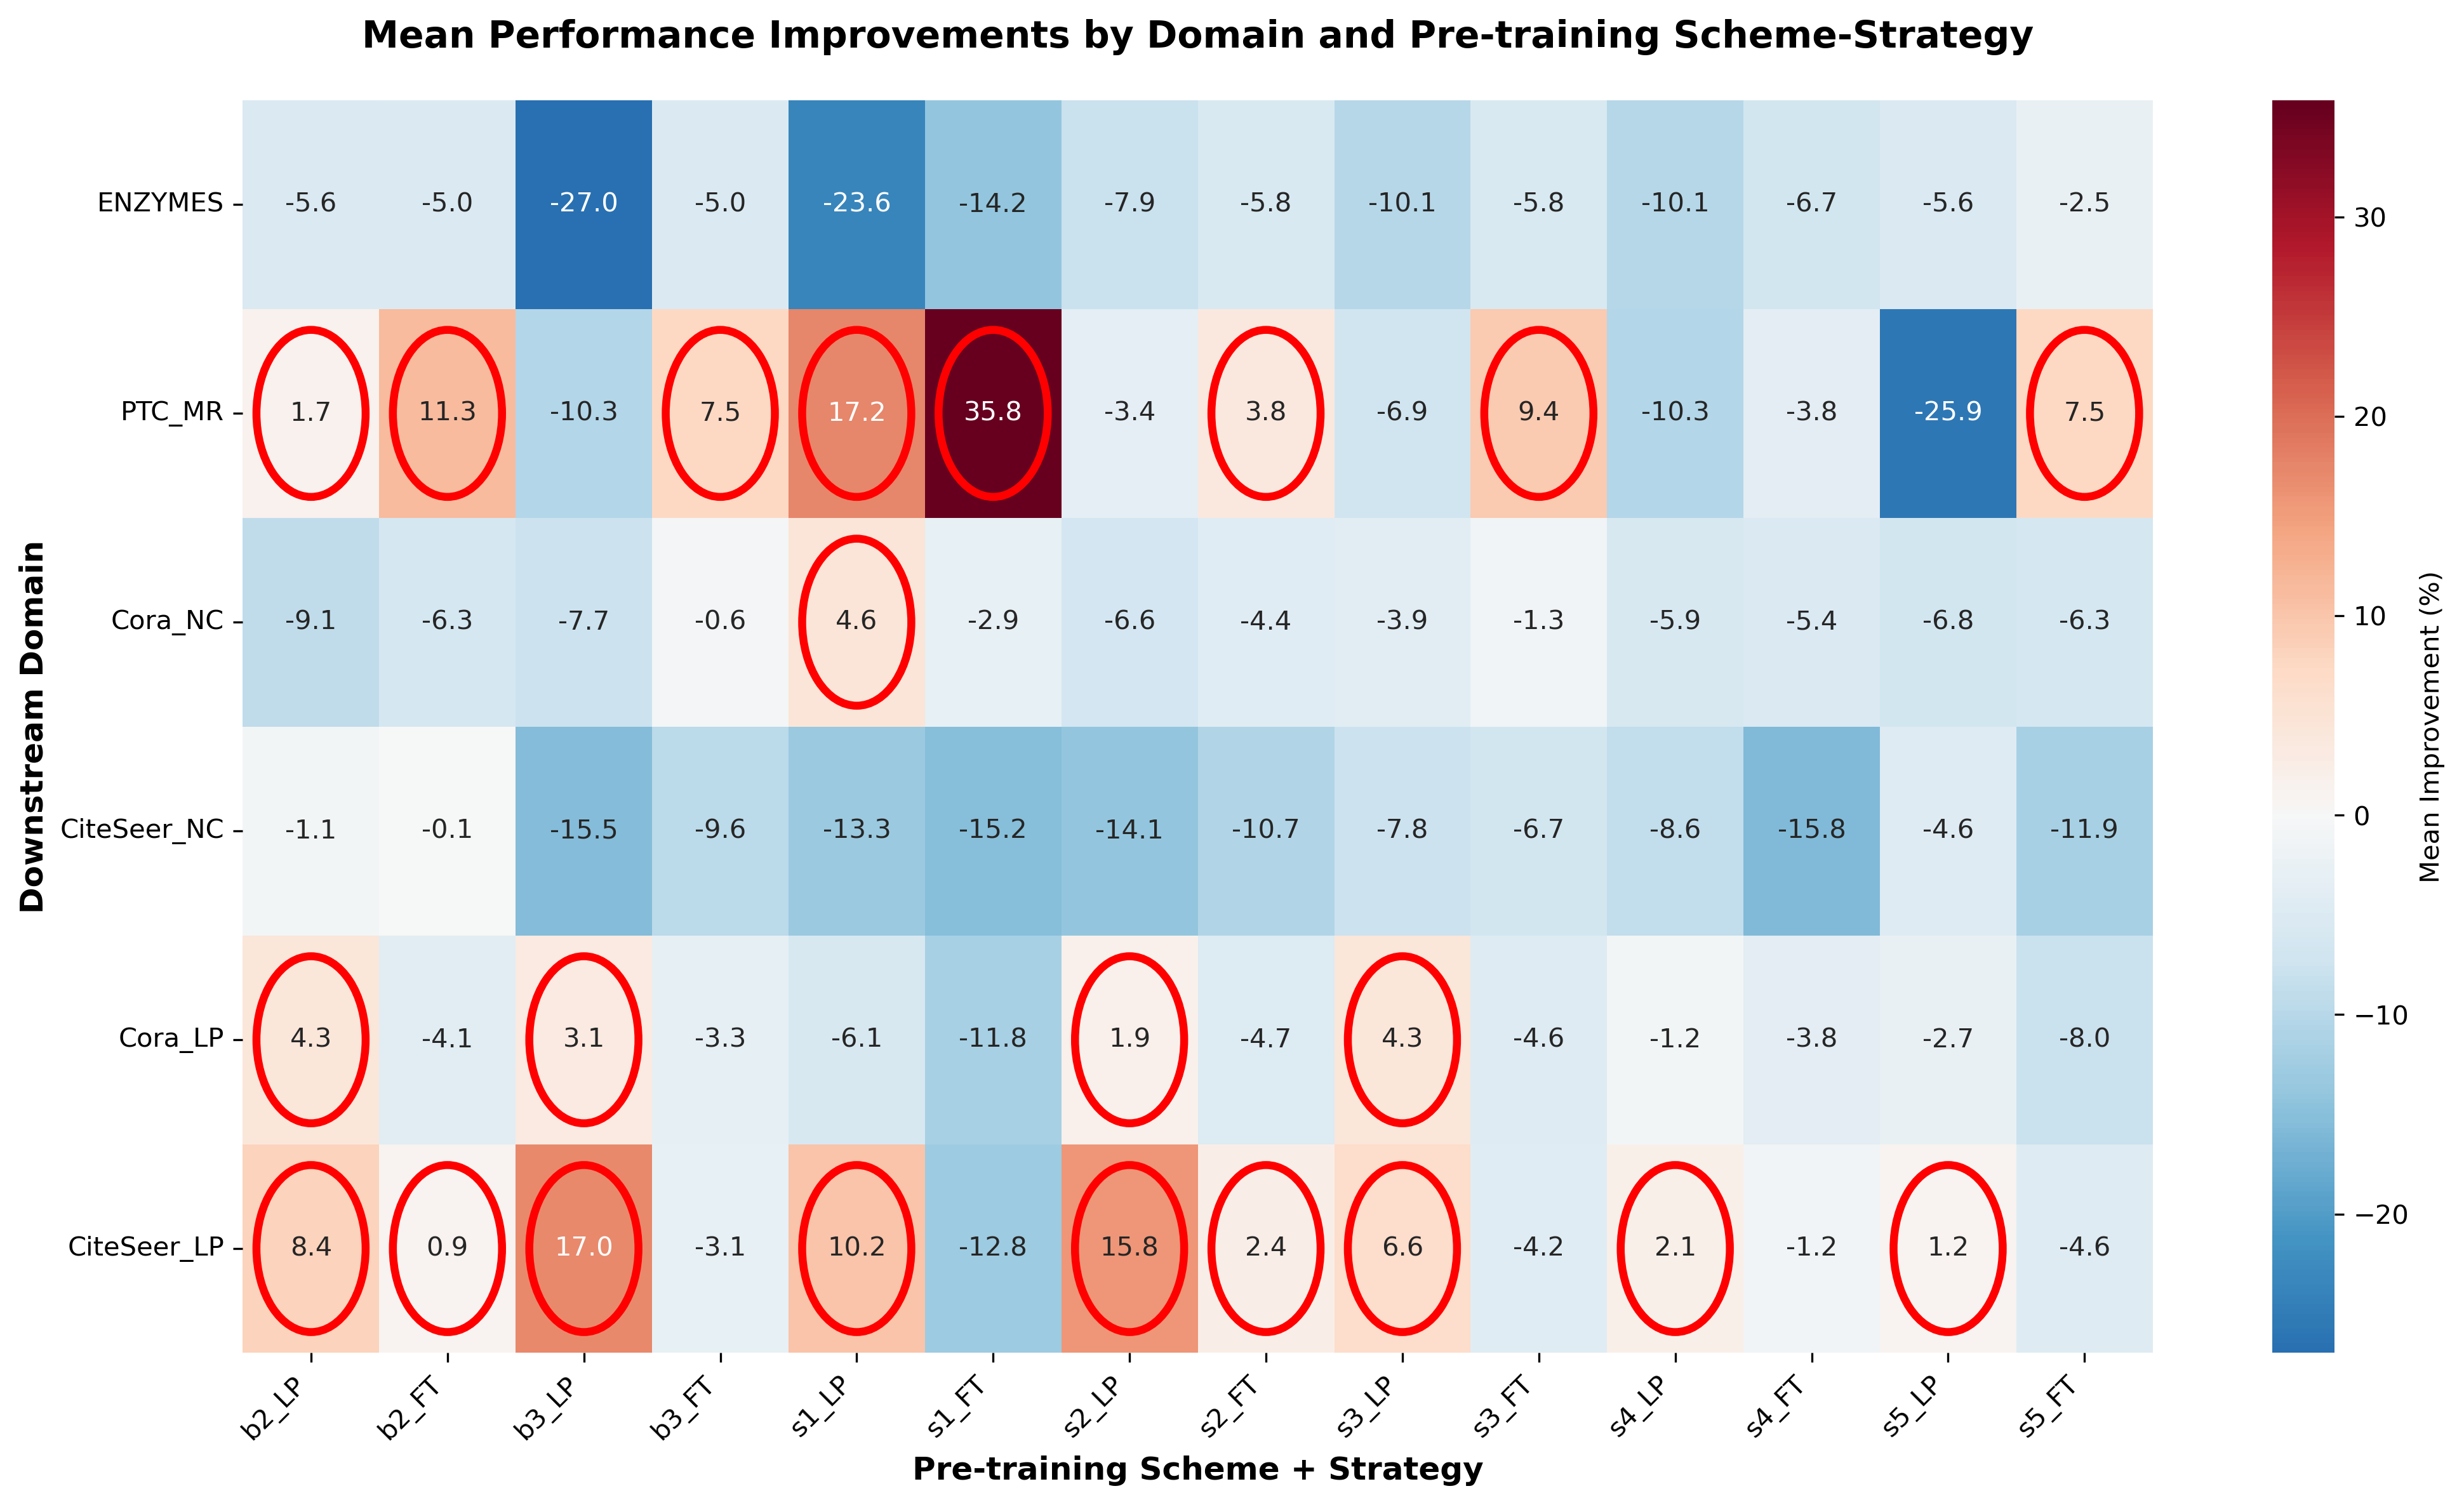
\includegraphics[width=0.9\textwidth]{domain_performance_heatmap.png}
\caption{Performance improvement heatmap by domain and pre-training scheme-strategy combinations. Red indicates positive improvements, blue indicates negative transfer. The selective nature of positive transfer is clearly visible, with molecular domains showing strong affinity for specific schemes (s1\_FT for PTC\_MR), while citation domains favor different combinations (b3\_LIN for link prediction tasks).}
\label{fig:domain-heatmap}
\end{figure*}

\begin{figure*}[!ht]
\centering
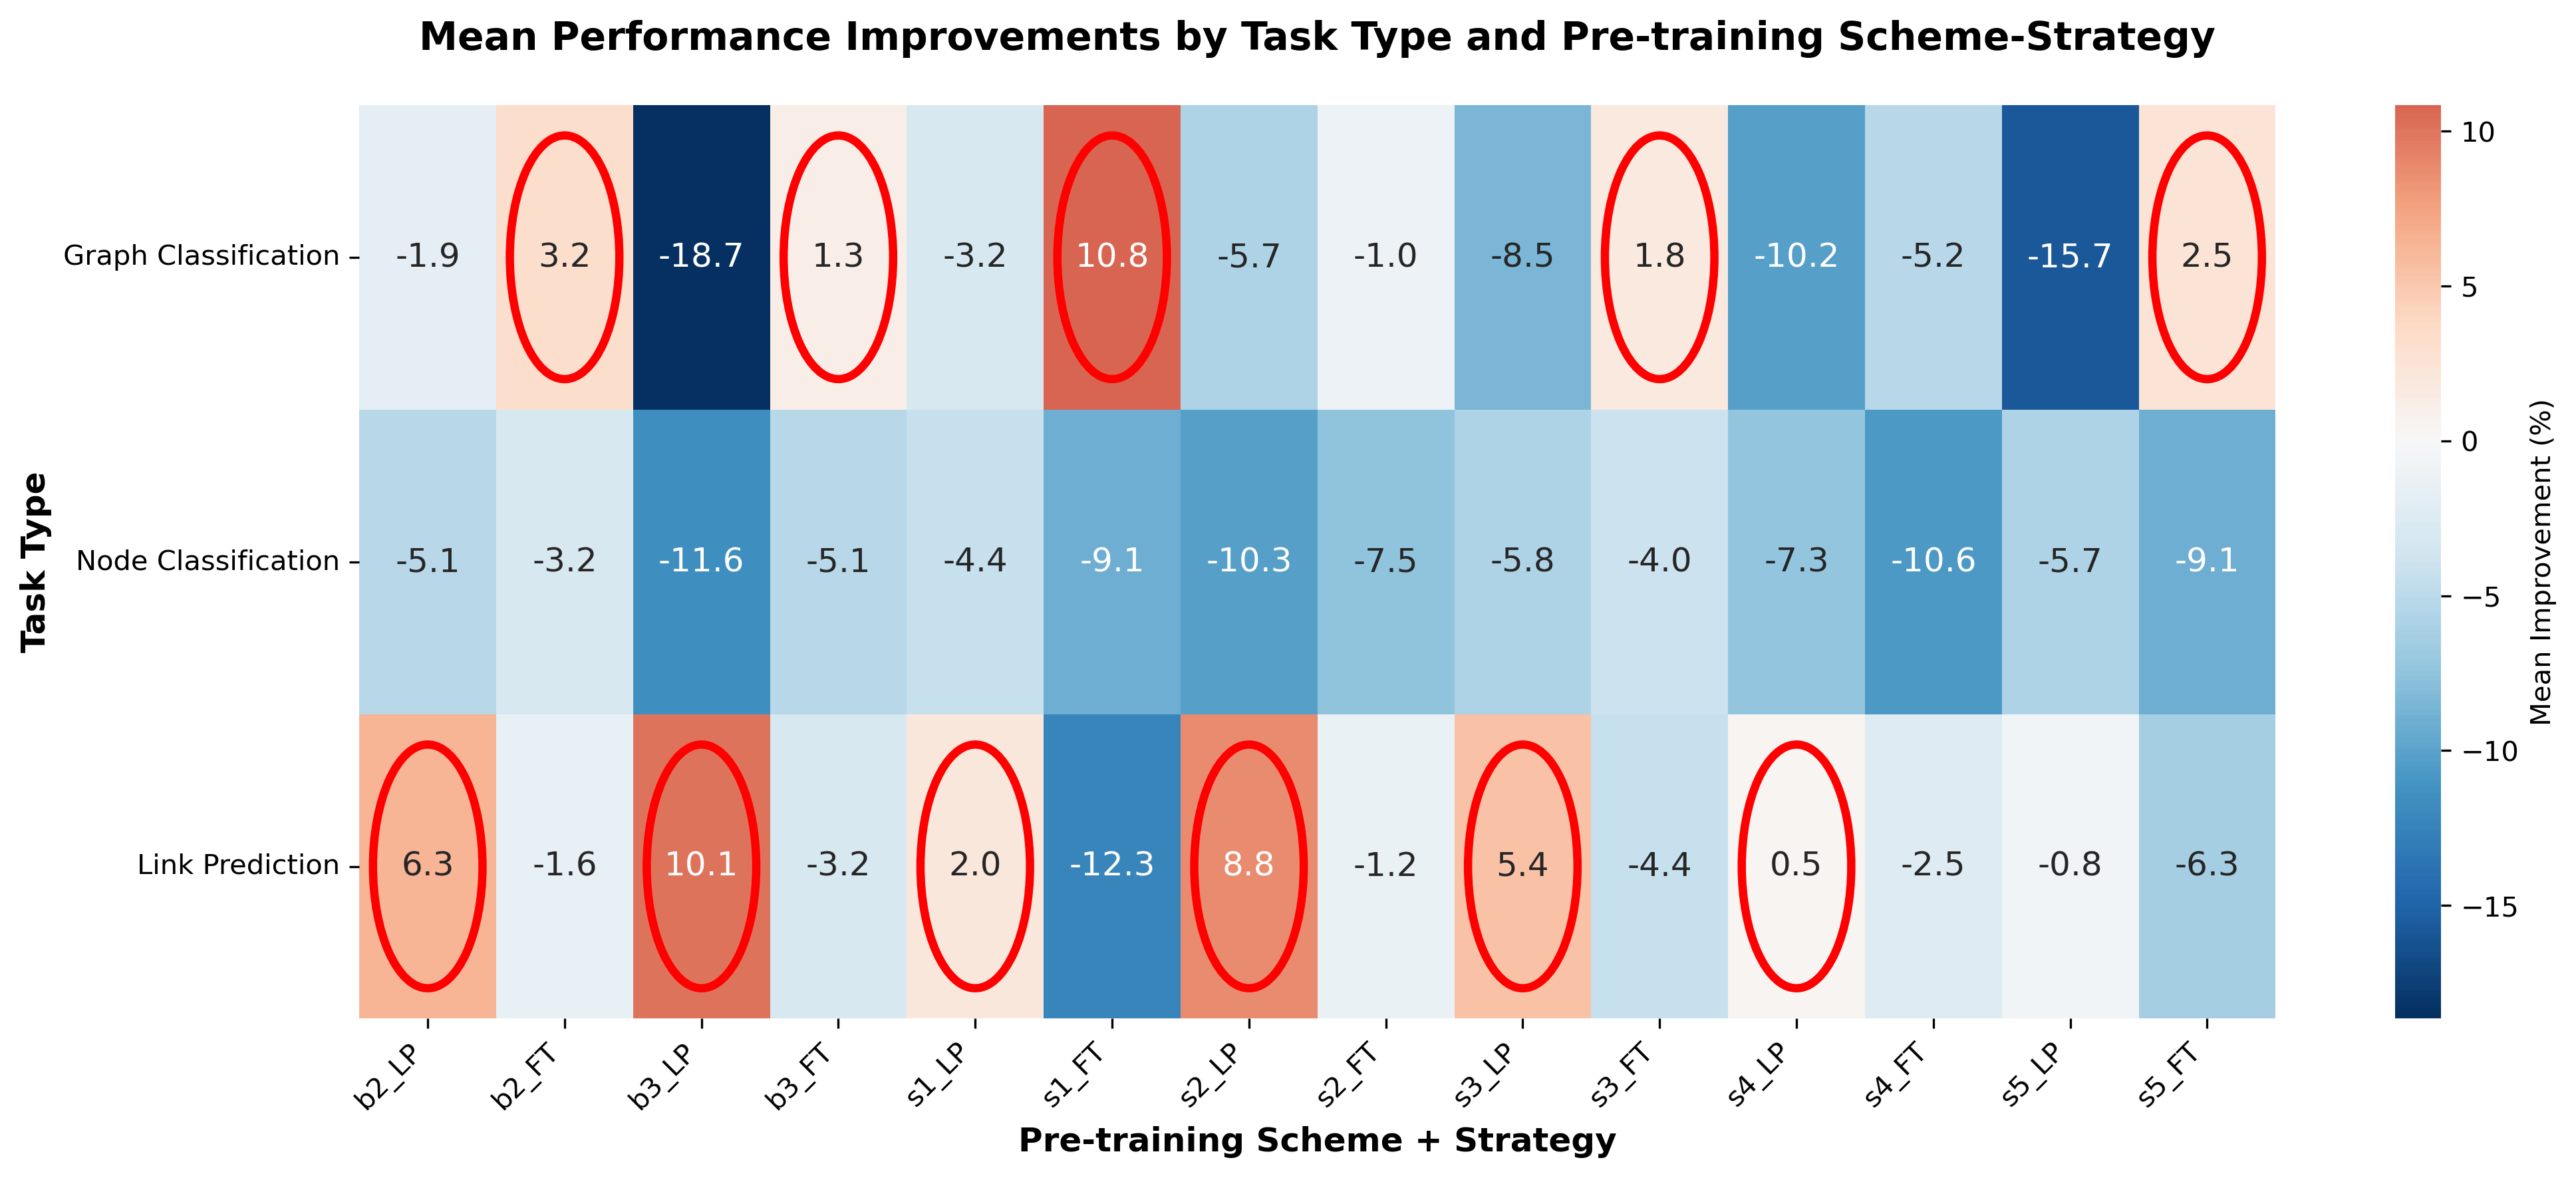
\includegraphics[width=0.9\textwidth]{task_type_performance_heatmap.png}
\caption{Performance improvement patterns by task type reveal systematic optimization guidelines. Graph Classification (GC) shows high variability with notable peaks (s1\_FT), Node Classification (NC) exhibits consistent modest negative transfers, while Link Prediction (LP) demonstrates reliable positive improvements with linear probing strategies (b3\_LinearProbe). These patterns enable task-type-first deployment protocols.}
\label{fig:task-heatmap}
\end{figure*}

\clearpage

% -------------------------
% Appendix
% -------------------------
\appendix

\section{Implementation Details}

\subsection{Architecture Specifications}

\paragraph{GNN Backbone.} We use a 5-layer Graph Isomorphism Network (GIN) with hidden dimension 256 throughout all layers. Each GIN layer contains an MLP: $[256 \rightarrow 512 \rightarrow 256]$ with BatchNorm and ReLU activation. Residual connections are applied: $h_{\text{out}} = \text{GINConv}(h) + h$. Dropout rate is 0.2 after each layer.

\paragraph{Task-Specific Heads.} Pre-training heads: Node Feature Masking $[256 \rightarrow 256 \rightarrow 256]$, Link Prediction $[768 \rightarrow 256 \rightarrow 1]$ (768 from concatenated edge features $[h_u + h_v + |h_u - h_v|]$), Node Contrastive $[256 \rightarrow 256 \rightarrow 128]$, Graph Contrastive $[512 \rightarrow 256 \rightarrow 128]$ (512 from mean+max pooling concatenation), Graph Properties $[256 \rightarrow 512 \rightarrow 12]$, Domain Classifier $[256 \rightarrow 128 \rightarrow 4]$ with 0.5 dropout.

\subsection{Training Hyperparameters}

\paragraph{Pre-training.} 50 epochs, batch size 32, gradient clipping (max norm 0.5), patience 50\% of total epochs. Task-specific learning rates: Link Prediction 5×10$^{-7}$, Node Feature Masking 1×10$^{-5}$, Node/Graph Contrastive 1×10$^{-5}$, Graph Properties 1×10$^{-5}$, Domain Adversarial 5×10$^{-6}$, weight decay 1×10$^{-5}$.

\paragraph{Fine-tuning.} Domain-specific epochs: molecular datasets (ENZYMES, PTC\_MR) 100 epochs; citation datasets 200-300 epochs. Batch sizes: molecular 32, node tasks full-batch, link prediction 256. Learning rates: backbone 1×10$^{-4}$ (if unfrozen), heads/encoders 1×10$^{-3}$. ENZYMES domain-adaptive encoder frozen during fine-tuning.

\subsection{Multi-task Learning Components}

\paragraph{PCGrad Gradient Surgery.} Tasks processed in shuffled order. Conflicting gradients projected: $g_i' = g_i - \frac{g_i \cdot g_j}{||g_j||^2} g_j$ when $g_i \cdot g_j < 0$. Final gradients averaged across tasks \citep{yu2020pcgrad}.

\paragraph{Adaptive Loss Balancing.} Warmup for 100 steps with equal weights. Inverse magnitude weighting: $w_i = \frac{1}{|L_i| + \varepsilon}$ where $\varepsilon = 10^{-8}$. Weights normalized to sum to 1.

\paragraph{Domain Adversarial Training.} Gradient Reversal Layer activates at 40\% training progress. Schedule: $\lambda = 2/(1 + \exp(-\gamma p)) - 1$ where $\gamma = 10$, $p$ is progress, maximum $\lambda = 0.01$.

\subsection{Pre-training Tasks}

\paragraph{Node Feature Masking.} Mask 15\% of nodes per graph (minimum 3). Learnable mask token initialized $\mathcal{N}(0, 0.01^2)$. MSE reconstruction loss on masked positions.

\paragraph{Graph Augmentation.} Node dropping (20\% rate, always applied), edge dropping (20\% probability, 20\% rate), attribute masking (20\% probability, 20\% rate). Minimum constraints: 3 nodes, 3 edges, 3 features.

\paragraph{Contrastive Learning.} Temperature annealing: $T(t) = T_{\text{init}} \cdot (T_{\text{final}}/T_{\text{init}})^{t/T_{\text{max}}}$ where $T_{\text{init}} = 0.5$, $T_{\text{final}} = 0.2$. Hard negative mining: 30\% of negatives, minimum 8 hard negatives based on embedding similarity.

\subsection{Data Processing}

\paragraph{Dataset Splits.} Pre-training: 90\% train, 10\% validation. Fine-tuning: 80\% train, 10\% validation, 10\% test. Stratified splitting for molecular datasets, random for citation node classification domains, and standard for citation link prediction domains.

\paragraph{Graph Properties (12-dimensional).} Number of nodes/edges, density, degree statistics (mean, variance, maximum), clustering coefficient, transitivity, connected components count, diameter, degree assortativity, degree centralization.

\paragraph{Feature Scaling.} StandardScaler fit on training data. Continuous datasets (ENZYMES) scaled and clipped to [-3, 3].

\subsection{Evaluation Protocol}

\paragraph{Metrics.} Graph/Node Classification: accuracy, F1, precision, recall. Link Prediction: AUC, accuracy, F1, precision, recall. Binary tasks use probabilities from output column 1. Multi-class uses macro-averaged metrics.

\paragraph{Statistical Setup.} Seeds: 42, 84, 126. Deterministic training: \\\texttt{torch.backends.cudnn.deterministic = True}. Early stopping on validation AUC (link prediction) or accuracy (classification) with 50\% patience.

\paragraph{Hardware.} All experiments on CUDA-enabled GPUs. PyTorch 1.12+, PyTorch Geometric 2.0+. Models implemented with AdamW optimizer ($\beta_1 = 0.9$, $\beta_2 = 0.999$, $\varepsilon = 10^{-8}$).

\section{Pre-training Task Technical Details}
\label{sec:pretrain-tasks}

Our framework employs six distinct self-supervised pre-training tasks, each targeting different aspects of graph representation learning. We provide detailed technical descriptions below.

\subsection{Node Feature Masking (NFM)}
\label{sec:nfm}

Node Feature Masking follows a mask-and-reconstruct paradigm similar to BERT \citep{devlin2019bert}:

\begin{enumerate}
\item \textbf{Masking Strategy:} For each graph, randomly select 15\% of nodes (minimum 3 nodes). Replace selected node features with a learnable mask token $\mathbf{m} \in \mathbb{R}^d$.

\item \textbf{Reconstruction:} Apply domain-adaptive encoder first, then mask selected features, then GNN backbone: $\mathbf{H} = \text{GNN}(\mathbf{H}_{\text{masked}}, \mathbf{A})$ where $\mathbf{H}_{\text{masked}}$ contains mask tokens at selected positions

\item \textbf{Loss Function:} Minimize MSE between original and reconstructed features:
\begin{equation*}
\mathcal{L}_{\text{NFM}} = \frac{1}{|M|} \sum_{v \in M} ||\text{MLP}_{\text{recon}}(\mathbf{h}_v) - \mathbf{h}_v^{\text{orig}}||^2
\end{equation*}
where $M$ is the set of masked nodes and $\text{MLP}_{\text{recon}}$ is a domain-specific reconstruction head.
\end{enumerate}

\subsection{Link Prediction (LP)}
\label{sec:lp}

Link Prediction trains the model to distinguish existing edges from non-existing ones:

\begin{enumerate}
\item \textbf{Positive Sampling:} Use all edges in the original graph as positive samples.

\item \textbf{Negative Sampling:} Generate equal number of negative edges using uniform sampling, ensuring no overlap with existing edges.

\item \textbf{Edge Representation:} For edge $(u,v)$, compute:
\begin{equation*}
\mathbf{e}_{u,v} = [\mathbf{h}_u + \mathbf{h}_v; \mathbf{h}_u \odot \mathbf{h}_v; |\mathbf{h}_u - \mathbf{h}_v|]
\end{equation*}
where $[;]$ denotes concatenation and $\odot$ is element-wise product.

\item \textbf{Loss Function:} Binary cross-entropy over all edge pairs:
\begin{align*}
\mathcal{L}_{\text{LP}} &= -\frac{1}{|E|} \sum_{(u,v)} \big[ y_{u,v} \log \sigma(f(\mathbf{e}_{u,v})) \\
&\quad + (1-y_{u,v}) \log(1-\sigma(f(\mathbf{e}_{u,v}))) \big]
\end{align*}
where $f(\cdot)$ is the MLP predictor.
\end{enumerate}

\subsection{Node Contrastive Learning}
\label{sec:node-contrast}

Node-level contrastive learning using graph augmentations:

\begin{enumerate}
\item \textbf{Augmentation Strategy:} Create two views of each graph through:
\begin{itemize}
\item Node dropping (20\% rate, minimum 3 nodes retained)
\item Edge dropping (20\% probability, 20\% rate, minimum 3 edges retained)  
\item Attribute masking (20\% probability, 20\% features)
\end{itemize}

\item \textbf{Common Node Identification:} Find nodes present in both augmented views for contrastive pairing.

\item \textbf{Projection:} Apply domain-specific projection head: $\mathbf{z}_v = \text{MLP}_{\text{proj}}(\mathbf{h}_v)$

\item \textbf{NT-Xent Loss:} For node $v$ with augmented views $\mathbf{z}_v^{(1)}, \mathbf{z}_v^{(2)}$:
\begin{align*}
\mathcal{L}_{\text{node}} &= -\frac{1}{2N} \sum_{i=1}^{N} \left[ \log \frac{e^{s_{i,i}/\tau}}{\sum_{k \neq i} e^{s_{i,k}/\tau}} \right. \\
&\quad \left. + \log \frac{e^{s_{i,i}/\tau}}{\sum_{k \neq i} e^{s_{k,i}/\tau}} \right]
\end{align*}
where $s(\cdot,\cdot)$ is cosine similarity, $\tau$ is temperature, and the loss is computed symmetrically for both view directions.
\end{enumerate}

\subsection{Graph Contrastive Learning}
\label{sec:graph-contrast}

Graph-level contrastive learning operates on entire graph representations:

\begin{enumerate}
\item \textbf{Graph Representation:} Combine mean and max pooling:
\begin{equation*}
\mathbf{s}_G = [\text{MeanPool}(\mathbf{H}); \text{MaxPool}(\mathbf{H})]
\end{equation*}

\item \textbf{Augmentation:} Same strategy as node contrastive, but applied to generate two graph views.

\item \textbf{Loss Function:} Similar NT-Xent formulation but operating on graph-level representations instead of node embeddings.
\end{enumerate}

\subsection{Graph Property Prediction}
\label{sec:graph-prop}

Prediction of structural graph properties for self-supervised learning:

\begin{enumerate}
\item \textbf{Property Computation:} Extract 12 structural properties per graph:
\begin{itemize}
\item Basic: \#nodes, \#edges, density, degree statistics
\item Structural: clustering coefficient, transitivity, diameter
\item Advanced: assortativity, degree centralization, connected components
\end{itemize}

\item \textbf{Standardization:} Z-score normalize properties using training set statistics.

\item \textbf{Loss Function:} MSE regression over all properties:
\begin{equation*}
\mathcal{L}_{\text{prop}} = \frac{1}{|G|} \sum_{G_i} ||\text{MLP}_{\text{prop}}(\mathbf{s}_{G_i}) - \mathbf{p}_{G_i}||^2
\end{equation*}
where $\mathbf{s}_{G_i}$ is the mean pooling summary of all nodes in graph $G_i$ and $\mathbf{p}_{G_i}$ are the standardized properties of graph $G_i$.
\end{enumerate}

\subsection{Domain Adversarial Training}
\label{sec:domain-adv}

Domain adversarial training promotes domain-invariant representations:

\begin{enumerate}
\item \textbf{Gradient Reversal Layer:} Applies identity in forward pass, negates gradients in backward pass with scaling factor $\lambda$.

\item \textbf{Domain Classification:} Train classifier to predict source domain:
\begin{equation*}
\mathcal{L}_{\text{domain}} = -\frac{1}{|G|} \sum_{G_i} \log P(d_i | \text{GRL}(\mathbf{s}_{G_i}; \lambda))
\end{equation*}
where $\mathbf{s}_{G_i}$ is the mean pooling summary of all nodes in graph $G_i$, $d_i$ is the true domain label and GRL is gradient reversal.

\item \textbf{Schedule:} $\lambda$ increases from 0 to 0.01 using sigmoid schedule starting at 40\% of training.
\end{enumerate}

\section{Hyperparameter Details}

\subsection{Pre-training Configuration}
\begin{itemize}
\item Epochs: 50 with early stopping (patience: 50\% of total epochs)
\item Batch size: 32 graphs across all domains
\item Gradient clipping: max norm 0.5
\item Temperature scheduling: 0.5 $\rightarrow$ 0.2 (exponential decay)
\item Domain adversarial $\lambda$: 0 $\rightarrow$ 0.01 (sigmoid schedule, starting at 40\% training)
\end{itemize}

\subsection{Fine-tuning Configuration}
Task-specific configurations optimized through preliminary experiments:

\textbf{Molecular domains (ENZYMES, PTC\_MR):}
\begin{itemize}
\item Epochs: 100, Batch size: 32
\item Learning rates: Backbone 1e-4, Domain-adaptive encoder/Head 1e-3
\end{itemize}

\textbf{Citation domains (Cora, CiteSeer):}
\begin{itemize}
\item Node Classification: 200 epochs, full batch
\item Link Prediction: 300 epochs, batch size 256
\item Learning rates: Backbone 1e-4, Domain-adaptive encoder/Head 1e-3
\end{itemize}

\textbf{Linear Probing Setup:} Domain-adaptive encoder + classifier head training (GNN backbone frozen). Exception: ENZYMES domain-adaptive encoder also frozen due to in-domain pre-training.


\end{document}
